\section{A case solved exactly at every noise level}\label{sec:exact}

\paragraph{In brief.}
For a one-step fluctuating stage followed by a geometric steady stay, independent gamma-distributed host abundance permits an exact calculation. At every fixed positive host variance, lengthening the steady stay strictly reduces the threshold loss in this linear rare-parasite setting. With nonnegative host memory, the decrease is proved only to second order or, for the bounded two-state host, for long stays. Strongly negative memory can reverse it.

Time spent in a steady stage can reduce exposure to fluctuating transmission. Using \citet{roerdink1988}'s exact growth formula for a one-step fluctuating stage and a geometric steady stay, we prove that the threshold loss decreases strictly with the steady stay at every fixed gamma host variance.

\subsection{Model, invariant law, and attribution}\label{subsec:exact-model}

Stage~0 has no staying, and its transfer to stage~1 fluctuates with relative host abundance $h_t$. Stage~1 has staying fraction $s\in(0,1)$, mean stay $\tau=1/(1-s)$ steps, and constant transfer $g_1>0$ back to stage~0. With mean outward transfer $g_0>0$, product $c=g_0g_1>0$, and population vector $\mathbf{x}(t)=(x_0(t),x_1(t))^{\mathsf{T}}$, the map is
\begin{equation}
\begin{gathered}
\mathbf{x}(t+1) = \mathbf{A}(t)\mathbf{x}(t), \qquad
\mathbf{A}(t) = \begin{pmatrix} 0 & g_1 \\ g_0 h_t & s \end{pmatrix},\\
x_1(t+1) = s x_1(t) + c h_t x_1(t-1),
\end{gathered}
\label{eq:exact-matrix}
\end{equation}
where the host multipliers $h_t$ are independent and identically distributed across time steps $t$ according to a gamma law $\operatorname{Gamma}(p, 1/p)$ with shape parameter $p > 0$ and scale parameter $1/p$, so that $\mathbb{E} h_t = 1$ and $\operatorname{Var}(h_t) = 1/p$. All logarithms below are natural. The arithmetic-mean matrix has characteristic equation $\lambda^2 = s\lambda + c$ and deterministic per-circuit reproduction number $R_0 = c/(1-s)$, with mean-matrix threshold $c = 1-s$. Counting one transfer as birth, the stochastic threshold loss $D(s,p)$ is the logarithmic increase in $R_0$ required to restore zero long-run stochastic growth $r(s,c,p)$ from its mean threshold, defined implicitly along with the logarithmic gap $\ell(p)$ and the auxiliary ratio chain $X_t$ by
\begin{equation}
\begin{gathered}
r\bigl(s, (1-s)\mathrm{e}^{D(s,p)}, p\bigr) = 0,\\
\ell(p) = -\mathbb{E}\ln h_t = \ln p - \psi(p), \qquad
X_{t+1} = \frac{Y_{t+1}}{s + X_t},
\end{gathered}
\label{eq:exact-defs}
\end{equation}
where $\psi = \Gamma'/\Gamma$ is the digamma function, $\psi_1 = \psi'$ is the trigamma function (with $\operatorname{Var}(\ln h_t) = \psi_1(p)$), $\gamma$ denotes Euler's constant, $Y_t = c h_t \sim \operatorname{Gamma}(p, \theta)$ with scale $\theta = c/p$ is independent of the past, and $\kappa = s^2/\theta = s^2 p/c$ is the dimensionless ratio parameter. All numerical parameter values below are illustrative properties of this mathematical model rather than measurements on real parasites.

The exact solution is due to \citet{roerdink1988}, who studied the same matrix for biennial life histories with fluctuating recruitment. His equations~3.15a--3.16 give the invariant Kummer density, and his equation~5.6 gives the Tricomi growth formula. The invariant continued-fraction law goes back to \citet{dyson1953}, whose original equations were checked indirectly through later treatments \citep{roerdink1988,marklof2008,letac2010,forrester2021a,forrester2021b}. We use these published results to study the threshold after compensating for changes in the deterministic reproduction number.

An auxiliary population ratio has a unique stationary distribution, which gives the long-run growth rate for every nonzero nonnegative starting population (Proposition~\ref{prop:exact-R1}, Appendix~\ref{sec:exact-app}).

Independent quadrature checks of the growth formula are described in Online Resource~1.

Roerdink's exact growth formula can be evaluated using special functions or convergent series (Proposition~\ref{prop:exact-R2}, Appendix~\ref{sec:exact-app}).

In a general independent-environment ring (Section~\ref{sec:bounds}), Jensen's inequality gives only the weak bounds $0 \le D \le \ell(p)$. For the gamma cycle with interior staying, both inequalities are strict at every noise amplitude (proved in Appendix~\ref{sec:exact-app} and refereed).

\begin{proposition}\label{prop:exact-R3}
For every $s \in (0,1)$ and every $p > 0$, the growth rate $r(s,c,p)$ is continuous and strictly increasing in $c \in (0,\infty)$, with $\lim_{c\downarrow 0} r(s,c,p) = \ln s < 0$ and $\lim_{c\to\infty} r(s,c,p) = \infty$. Consequently, there exists a unique real root $D(s,p)$ of $r(s, (1-s)\mathrm{e}^y, p) = 0$, and it satisfies
\begin{equation}
0 < D(s,p) < \ell(p).
\label{eq:exact-bounds}
\end{equation}
\end{proposition}

Any $s>0$ recovers part of the logarithmic-gap penalty, while variability still imposes a positive cost. Constant survival in the storage stage matters. With gamma noise on the staying entry instead, the companion random-matrix model has $D_{\mathrm{stay}}>0$ and $D_{\mathrm{stay}}\to\infty$ as $s\uparrow1$ at fixed $p$ (Proposition~\ref{prop:exact-R8}; proved and refereed). The unbounded multiplier is not a survival probability; details are in Online Resource~1.

The exact loss and second-order approximation are compared in Fig.~\ref{fig:exact-1}; numerical details are in Online Resource~1.

\begin{figure}[t]
\centering
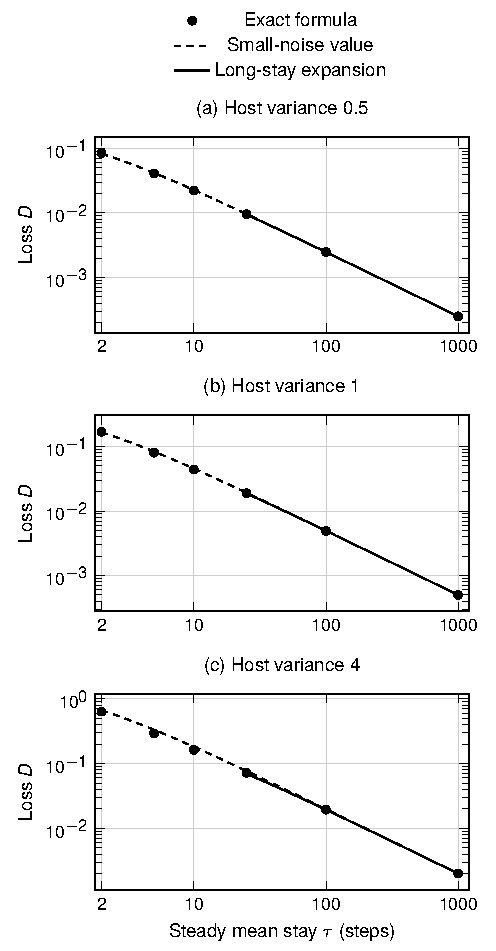
\includegraphics[width=84mm]{figures/exact-1.pdf}
\caption{Threshold loss against steady mean stay $\tau$ for illustrative host variances \textbf{(a)}~$0.5$, \textbf{(b)}~$1$, and \textbf{(c)}~$4$. Filled circles are exact-formula roots at stays $2,5,10,25,100,1000$ (validation in Online Resource~1). Dashed curves give the second-order small-noise value $Q=1/[2p(1+\tau)]$. Solid curves for $\tau\geq25$ give the two-term long-stay expansion in Proposition~\ref{prop:exact-R6}. All axes are logarithmic}\label{fig:exact-1}
\end{figure}

\subsection{Endpoint regimes and non-commuting normalized limits}\label{subsec:exact-asymptotics}

Without staying, two separate two-step cohorts each incur the full logarithmic gap $\ell(p)$. At fixed host variance, the loss approaches this endpoint at an inverse-logarithmic rate as staying tends to zero (Proposition~\ref{prop:exact-R5}, Appendix~\ref{sec:exact-app}; refereed).

The inverse-logarithmic deficit means that even very small retention reduces threshold loss (Fig.~\ref{fig:exact-2}; evaluated examples in Online Resource~1).

At long stays, the second-order approximation $Q=1/[2p(1+\tau)]$ becomes exact asymptotically at each fixed host variance (proved in Appendix~\ref{sec:exact-app}; refereed).

\begin{proposition}\label{prop:exact-R6}
Fix $p > 0$, and let $\varepsilon = 1 - s = 1/\tau$. As $\varepsilon \downarrow 0$,
\begin{equation}
\begin{split}
D(s,p) &= \frac{\varepsilon}{2p} - \frac{12p + 7}{24 p^2}\varepsilon^2 + O_p(\varepsilon^3),\\
\frac{D(s,p)}{1/[2p(1+\tau)]} &= 1 - \frac{7}{12 p \tau} + O_p(\tau^{-2}) \longrightarrow 1.
\end{split}
\label{eq:exact-long-stay}
\end{equation}
\end{proposition}

Proposition~\ref{prop:exact-R6} fixes $p$ and does not give a uniform double limit as $p\downarrow0$. Near zero staying, $Q$ understates $D$, so the small-noise expansion is not uniform in $s$ (proved in Appendix~\ref{sec:exact-app}; refereed). Numerical comparisons are in Online Resource~1.

\begin{figure}[t]
\centering
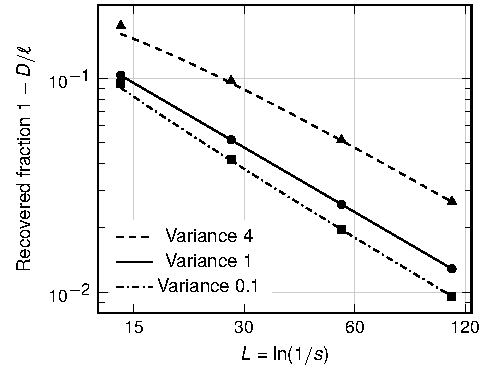
\includegraphics[width=84mm]{figures/exact-2.pdf}
\caption{Fraction of the logarithmic-gap upper bound recovered by small staying, $1 - D(s,p)/\ell(p)$, against $L = \ln(1/s)$ on logarithmic axes for illustrative host variances $1/p = 4$ ($p = 1/4$, upward triangles and dashed curve), $1/p = 1$ ($p = 1$, circles and solid curve), and $1/p = 0.1$ ($p = 10$, squares and dash-dotted curve). Markers show exact-formula evaluations at $s = 10^{-6}, 10^{-12}, 10^{-24}, 10^{-48}$ (validation in Online Resource~1), and curves show the two-term inverse-logarithm asymptotic $\psi_1(p)/(2\ell L) + \psi_1(p)[\psi(p)+\gamma]/(2\ell L^2)$ of Proposition~\ref{prop:exact-R5}, whose $L^{-2}$ term vanishes at $p = 1$}\label{fig:exact-2}
\end{figure}

Taking small noise and vanishing staying in opposite orders gives different limits after dividing loss by host variance (Proposition~\ref{prop:exact-R7}, Appendix~\ref{sec:exact-app}).

The normalized limits differ by a factor of two. Agreement with $Q$ at a fixed small stay can require very small noise (examples in Online Resource~1).

\subsection{Strict decrease of the loss with residence time at every noise level}\label{subsec:exact-theorem}

The endpoint expansions give decrease near both ends at each fixed $p$. To settle intermediate stays, we express the derivative as a covariance (proved in Appendix~\ref{sec:exact-app}; refereed).

\begin{proposition}\label{prop:exact-R4}
For $p>0$, let $T$ have density proportional to $t^{p-1}(1+t)^{-p}\mathrm{e}^{-\kappa t}$ on $t>0$, with $\kappa>0$, and put $W=\ln(1+T)$. The following parametrization covers the entire zero-growth curve $0<s<1$:
\begin{equation}
\begin{gathered}
m_p(\kappa) = \mathbb{E} W, \qquad s = \mathrm{e}^{-m_p(\kappa)},\\
V_p(\kappa) = \kappa\operatorname{Cov}(W, T) > 0,\\
g(p,\kappa) = \frac{\mathrm{d}D}{\mathrm{d}L} = \frac{1}{V_p(\kappa)} - 2 - \frac{s}{1-s},
\end{gathered}
\label{eq:exact-param}
\end{equation}
where $L=-\ln s=m_p(\kappa)$. The loss is real analytic in $s$. Its derivative is strictly negative everywhere if and only if $V_p(\kappa)<(1-s)/(2-s)$ for every $\kappa>0$.
\end{proposition}

Positivity of the covariance alone does not give the upper bound. The next theorem establishes it using a single-crossing property of the reflected density (proved in Appendix~\ref{sec:exact-app}; independently refereed as sound). Numerical evaluations illustrate the derivative but do not enter the proof.

\begin{theorem}\label{thm:exact-mono}
In the two-stage gamma model of equations~\eqref{eq:exact-matrix}--\eqref{eq:exact-defs} with $g_0, g_1 > 0$ and independent $h_t \sim \operatorname{Gamma}(p, 1/p)$, for every $p > 0$ and every $\kappa > 0$,
\begin{equation}
0 < V_p(\kappa) < \frac{1 - s}{2 - s}, \qquad s = \mathrm{e}^{-m_p(\kappa)}.
\label{eq:exact-mono}
\end{equation}
Consequently, for every $p > 0$, the threshold loss $D(s,p)$ is real analytic on $s \in (0,1)$ and satisfies $\partial_s D(s,p) < 0$ everywhere, so $D$ decreases strictly as the steady mean residence time $\tau = 1/(1-s) \in (1,\infty)$ increases. Furthermore, for each fixed $p > 0$, the logarithmic derivative $g(p,\kappa) = \mathrm{d}D/\mathrm{d}L > 0$ satisfies $\inf_{\kappa > 0} g(p,\kappa) = 0$ (unattained, with $g(p,\kappa) \sim \psi_1(p)/(2L^2) \to 0$ as $s \downarrow 0$ and $\lim_{\kappa\to\infty} g(p,\kappa) = 1/(2p)$), while for all sufficiently large $p$, $g(p,\cdot)$ has a unique local minimum on $\kappa \in [1/8, 1/2]$ at $\kappa_p = 1/4 + O(p^{-1/2})$, corresponding to $s_p = 1/(2\sqrt{p}) + O(p^{-1})$ and $g(p,\kappa_p) = 1/(8 p^{3/2}) + O(p^{-2})$.
\end{theorem}

The proof combines a strict Jensen-gap bound under integrability and single-crossing hypotheses (Proposition~\ref{prop:exact-P2}), verification for $W$ (Proposition~\ref{prop:exact-P3}), and a first-zero argument for $F=(2-s)V-(1-s)$ using the differential identities of Proposition~\ref{prop:exact-P1}. The appendix gives the full argument and endpoint expansions. The stated interior minimum is local, with no uniqueness claim outside the large-$p$ interval (Fig.~\ref{fig:exact-3}; proof outline in Online Resource~1).

\begin{figure}[t]
\centering
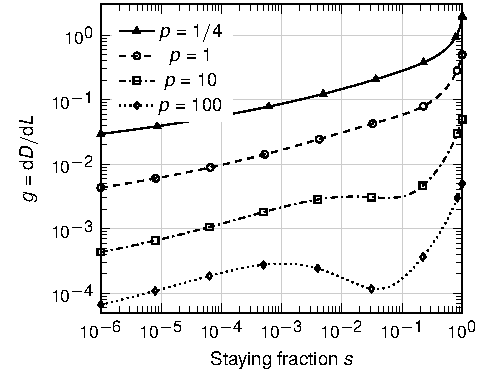
\includegraphics[width=84mm]{figures/exact-3.pdf}
\caption{Positive logarithmic derivative $g=\mathrm{d}D/\mathrm{d}L$, with $L=-\ln s$, against staying fraction $s$ for $p=1/4$ (solid, open triangles), $p=1$ (dashed, open circles), $p=10$ (dash-dotted, open squares), and $p=100$ (dotted, open diamonds). Each curve consists of 121 evaluations of the exact parametric formula in Proposition~\ref{prop:exact-R4}, with markers distinguishing the shapes. Both axes are logarithmic. The interior dips at the larger shapes do not attain the global infimum, which is zero as $s\downarrow0$}\label{fig:exact-3}
\end{figure}

\subsection{Hosts with memory}\label{subsec:exact-memory}

Host memory changes the question because the current host can be associated with the population's past stage distribution. A separate derivation, now refereed by a second independent reviewer, treats the same recurrence with a mean-one lognormal host $h_t=\exp(\sigma\xi_t-\sigma^2/2)$. Here $\xi_t$ is a centered, stationary, ergodic, unit-variance Gaussian process with covariance $\rho(j)$. For every fixed $0<s<1$, putting $q=1-s$, the derivation gives
\begin{equation}
 D=\sigma^2F_\rho(s)+O_s(\sigma^4),\qquad
 F_\rho(s)=\frac{q}{2(1+q)}
 \left[1+2\sum_{j\geq1}(-q)^{j-1}\rho(j)\right].
 \label{eq:exact-memory-coefficient}
\end{equation}
The remainder and its first $s$ derivative are uniform on compact subintervals of $0<s<1$. The series and its interior $s$ derivatives converge absolutely without covariance summability. Without ergodicity, the result concerns the zero of the expected growth exponent, not a common almost-sure threshold. The coefficient and the $2-\sqrt5$ boundary below were independently re-derived in the referee check (proofs in Appendix~\ref{subsec:exact-app-memory}). For a Gaussian first-order autoregressive process with $\rho(j)=\phi^j$, $-1<\phi<1$,
\begin{equation}
\begin{split}
 F_\phi(s)&=\frac{q[1+(q+2)\phi]}{2(1+q)(1+q\phi)},\\
 \partial_sF_\phi&=-\frac{1+2\phi+2q\phi-q^2\phi^2}
 {2(1+q)^2(1+q\phi)^2}.
\end{split}
 \label{eq:exact-memory-AR}
\end{equation}
For $2-\sqrt5\leq\phi<1$ the derivative is negative at every interior stay. For $-1/2<\phi<2-\sqrt5$ it is negative exactly when $s>1-[1-\sqrt{2(1+\phi)}]/\phi$, vanishes at that boundary, and is positive below it. For $-1<\phi\leq-1/2$ it is positive throughout.

The ring comparisons depend on which stage has staying (Proposition~\ref{prop:ring-steady}). Let $a$ and $b$ denote the fluctuating and steady mean stays. Roerdink's model has $a=1$: neither adding a steady stage with $b>1$ nor lengthening it raises the second-order loss for $0\leq\phi<1$. Proposition~\ref{prop:exact-mem-ring} in Appendix~\ref{sec:exact-app} gives the addition threshold $b<a(2a-1)\theta/(a+\theta)$, where $\theta=\phi/(1-\phi)$. With sufficiently strong positive memory, exceeding the one-stage loss requires $a>1$, whereas a rise with $b\geq1$ requires $a>(3+\sqrt{17})/4$. A third stage also permits a rise: in $(1,b,c_3)$ it occurs at short $b$ for $\phi$ near one exactly when $c_3>2$. The three-stage numerical study uses $c_3=5$ (Online Resource~1). This coefficient result does not determine every finite-amplitude curve.

The refereed derivation also proves finite-amplitude results for the bounded symmetric Markov host $h_t=1+\delta Z_t$, $0<\delta<1$, where $Z_t\in\{-1,1\}$ is stationary and $\mathbb P(Z_{t+1}=Z_t)=(1+\phi)/2$, $-1<\phi<1$. It establishes a unique invariant environment--ratio law and threshold, with $D<\ell=-\tfrac12\ln(1-\delta^2)$, and $D>0$ when $0\leq\phi<1$. At each fixed $(\delta,\phi)$, for $\varepsilon=1-s$,
\begin{equation}
 \begin{split}
 D&=A\varepsilon+B\varepsilon^2+O_{\delta,\phi}(\varepsilon^3),\\
 A&=\delta^2(1/2+\phi),\qquad
 B=-\delta^2(1/2+\phi+\phi^2)+\tfrac32A^2.
 \end{split}\label{eq:exact-memory-long}
\end{equation}
For $A\ne0$, $0<\varepsilon<|A|/262144$ ensures $\operatorname{sign}D'(s)=-\operatorname{sign}A$ and $|D'(s)+A|<|A|/2$. In particular, $\delta=1/2$, $\phi=-3/4$, and $s=1-10^{-8}$ give the proved counterexample $D'(s)>1/32$. Two deterministic methods checked the counterexamples at 80-digit working precision (details in Online Resource~1). The small-staying correction is now proved in Appendix~\ref{subsec:exact-app-memory} and checked by a second party.

For the bounded two-state host, the loss again approaches the logarithmic penalty as staying tends to zero, with a correction that depends on host memory (Proposition~\ref{prop:exact-memory-small}, Appendix~\ref{sec:exact-app}).

For the stationary gamma value-refresh kernel with $p>0$, $0\leq\phi<1$, and the lognormal autoregressive host with $\sigma>0$, $|\phi|<1$, we also prove a unique threshold, $D<\ell=-\mathbb E\ln h_t$, $D>0$ for nonnegative memory, and finite-order long-stay expansions (Appendix~\ref{subsec:exact-app-memory}, checked by a second party with the stated fixes included). The full series in $\varepsilon=1-s$ has zero radius of convergence for both hosts, so these expansions are asymptotic, not convergent.

GAP~1 is partly closed by the following result, proved in Appendix~\ref{subsec:exact-app-gap1} and checked independently.
\begin{proposition}[Uniform decrease for long stays]\label{prop:exact-memory-uniform}
For the stationary symmetric Markov host \(h_t=1+\delta Z_t\), \(Z_t\in\{-1,1\}\), with transition probabilities \(P_{ij}=(1+\phi ij)/2\), \(0<\delta<1\), and \(0\leq\phi<1\),
\begin{equation}\label{eq:exact-memory-uniform}
 D'(s)<0\qquad\text{for}\qquad 4/\sqrt{17}\leq s<1.
\end{equation}
More generally, this holds whenever \(c_*(s)/s^2\leq1/30\).
\end{proposition}
The rest of the interval, \(0<s<4/\sqrt{17}\), remains open. GAP~2 is closed and GAP~3 partly closed. For the specified unbounded hosts, memA P5's explicit derivative interval, P6's small-staying limit, and P7's noise holomorphy remain open, as does positivity for other correlated gamma kernels.

\begin{remark}[Interval certification]\label{rem:exact-certification}
GAP~4 is closed for the reported bounded-host computations, proof constants, 16 alternating-host cases, finite-state Gaussian calculations, and saved-table arithmetic, with independent checks and corrected values in Appendix~\ref{subsec:exact-app-certification}. The saved estimates classify 112 of 112 two-stage grids as decreasing and 15 of 24 three-stage grids as nonmonotone. Continuous Gaussian discretization and stochastic simulation error remain uncertified. These counts supply neither simultaneous confidence bands nor guarantees between sampled stays (Online Resource~1).
\end{remark}

\subsection{Literature status, formal verification, and biological scope}\label{subsec:exact-scope}

The literature audit distinguishes the exact solution from its threshold consequences. Roerdink's growth formula, invariant law, series, and leading small-staying growth expansion are published results \citep{roerdink1988}. The leading threshold correction and the normalized small-noise limits follow from those formulas. The audit did not find the compensated threshold analysis, strict bounds, higher small-staying corrections, long-stay expansion, or global monotonicity result in the 25 full-text documents it examined. Five target full texts, including Dyson's original, were not obtained directly. This states the scope of that search and does not establish universal priority.

Lean~4 checks the complete statements of Propositions~\ref{prop:exact-P1}, \ref{prop:exact-P2}, \ref{prop:exact-P3}, and~\ref{prop:exact-P6} under the recorded model and textbook assumptions, as well as specified components of the other exact-case results. Invariant-process and population-growth identifications and several analytic and asymptotic conclusions remain outside the credited formal coverage. The scope and remaining gaps are recorded in the reconciled coverage inventory archived with the Lean sources (see Code availability).

For a parasite with a one-step fluctuating transmission stage, independent gamma hosts, and a geometric steady stage, lengthening the steady stay strictly reduces threshold loss. The long-stay approximation holds at fixed gamma variance, with no uniform error claim as variance diverges. Host memory raises separate questions, as the bounded-host counterexample shows.
